\documentclass[conference]{IEEEtran}
\IEEEoverridecommandlockouts
\usepackage{cite}
\usepackage{amsmath,amssymb,amsfonts}
\usepackage{algorithmic}
\usepackage{graphicx}
\usepackage{textcomp}
\usepackage{xcolor}
\usepackage{booktabs}
\usepackage{listings}
\usepackage{tikz}

\def\BibTeX{{\rm B\kern-.05em{\sc i\kern-.025em b}\kern-.08em
    T\kern-.1667em\lower.7ex\hbox{E}\kern-.125emX}}
\begin{document}

\title{Hierarchical Multi-Agent Reinforcement Learning for Large-Scale Urban Traffic Orchestration over Real-World Networks\\
\thanks{Identify supporting technologies, institutions, and funding sources here if applicable.}
}

\author{\IEEEauthorblockN{Anonymous Authors}
\IEEEauthorblockA{\textit{Traffic Intelligence Research Laboratory} \\
\textit{Department of Computer Science and Engineering}\\
City, Country \\
email@example.com}
}

\maketitle

\begin{abstract}
Traffic congestion in rapidly expanding metropolises presents an immense challenge to classical static signal controllers and isolated optimization heuristics. In this work, we propose a Hierarchical Multi-Agent Reinforcement Learning (HMARL) framework designed to orchestrate urban traffic over highly realistic, real-world road networks. Our proposed system partitions traffic orchestration across three distinct spatial-temporal layers: a macro-level \textit{City Coordinator}, a meso-level \textit{Area Forecaster}, and a micro-level \textit{Ward Agent}. At the macro scale, the City Coordinator runs every 120 seconds, executing a Network Flow Linear Program across a multi-area topology to balance flows and restrict boundary inflows, preventing cascading gridlocks. At the meso scale, the Area Forecaster operates every 60 seconds, leveraging a Spatio-Temporal Graph Convolutional Network (STGCN) to project downstream ward congestion pressure. At the micro scale, decentralized Ward Agents execute Proximal Policy Optimization (PPO) policies on a 30-second decision cycle, mapping stacked temporal observations to high-level semantic actions that adaptively route traffic and prioritize emergency vehicles. We evaluate our system under realistic demographic models of Bengaluru traffic using the Simulation of Urban Mobility (SUMO) and the TraCI API. Our empirical results demonstrate that PPO-driven ward policies significantly outperform Deep Q-Networks (DQN) in highly stochastic environments, and that our full three-tier hierarchical coordination improves average vehicle speed by up to 34\% and reduces queue lengths by 42\% under extreme congestion scenarios.
\end{abstract}

\begin{IEEEkeywords}
Multi-agent reinforcement learning, hierarchical control, urban traffic simulation, spatio-temporal GCN, SUMO.
\end{IEEEkeywords}

\section{Introduction}
Traffic gridlock in modern metropolises leads to substantial economic and environmental costs. Rapid urbanization, particularly in dense, emerging cities like Bengaluru, India, leads to heterogeneous traffic profiles, extreme congestion hotspots, and high-frequency incident cascades. Traditional traffic management systems are highly inadequate in these environments. Standard implementations rely on localized fixed-time plans or simple adaptive signal controllers (e.g., SCATS, SCOOT) that operate on restrictive mathematical heuristics. These traditional systems fail to adapt to real-time traffic bursts, lack spatial coordination between neighboring intersections, and struggle to accommodate non-standard vehicle profiles (such as emergency vehicles and heavy freight trucks) alongside chaotic merging behavior.

In recent years, Reinforcement Learning (RL) has emerged as a promising paradigm for adaptive traffic control. By representing traffic junctions as learning agents, RL policies can dynamically adjust phase durations and coordinate flows in response to real-time observations. However, standard single-agent or flat multi-agent RL formulations suffer from major limitations when deployed at scale:
\begin{enumerate}
    \item \textbf{Dimensionality and Scalability Bottlenecks:} Modeling every single junction in a massive city network as an independent agent leads to an exponential growth in the state-action space, rendering joint policy optimization mathematically intractable.
    \item \textbf{Coordination Failure and Spillback propagation:} Decentralized flat agents often make conflicting local decisions. An agent at one junction may aggressively clear its local queues, only to dump a massive wave of vehicles directly into a downstream bottleneck, causing severe spillback and network deadlocks.
    \item \textbf{Sim-to-Real Gap:} Standard RL literature heavily simplifies road networks into synthetic grids (e.g., $3 \times 3$ Manhattan grids) and assumes uniform vehicle types, completely ignoring the complex topological morphology and diverse vehicle dynamics of actual urban layouts.
\end{enumerate}

To overcome these constraints, this work proposes a comprehensive, academically rigorous, and production-tested \textbf{Hierarchical Multi-Agent Reinforcement Learning (HMARL)} traffic management framework. Our system decomposes the complex global city traffic optimization problem into a three-tiered spatial-temporal control hierarchy:
\begin{itemize}
    \item \textbf{Micro-Scale Ward Agents:} Operate at a fine-grained, localized level. Each ward agent manages a cluster of intersections, mapping 30-timestep stacked observations to a discrete semantic action space consisting of 10 high-level traffic routing policies.
    \item \textbf{Meso-Scale Area Forecasters:} Coordinate groups of adjacent ward agents. An Area Forecaster leverages a PyTorch-based Spatio-Temporal Graph Convolutional Network (STGCN) to ingest localized temporal summaries and forecast boundary pressure values, shaping the micro-level reward signals.
    \item \textbf{Macro-Scale City Coordinator:} Acts as a strategic city-wide meta-controller. It executes a network-flow linear program (LP) over the inter-area connectivity graph every 120 seconds, issuing capacity bounds that throttle ingress flows and isolate cascading congestion.
\end{itemize}

Crucially, our system interfaces directly with realistic OpenStreetMap (OSM) data representing Bengaluru's most congested districts, including HSR Layout and BTM Layout. Using a robust preprocessing and simulation pipeline, we standardise geographic networks and stochastically generate demand profiles containing heterogeneous vehicle types (ambulances, BMTC buses, freight trucks, aggressive drivers, and slow drivers) and real-time incident cascades.

The remainder of this paper is structured as follows. Section II presents the theoretical foundations of the RL algorithms analyzed. Section III describes the simulator coupling and TraCI abstractions. Section IV details the map extraction and preprocessing pipeline. Section V explains the route generation and scenario modeling. Section VI highlights the topology stitching and connectivity logic. Section VII breaks down the hierarchical architecture and multi-scale temporal ticks. Section VIII details the semantic action space and overhauled reward formulation. Section IX presents the evaluation framework and benchmarking results, followed by conclusions and future work in Section X.

\section{Theoretical Foundations of Reinforcement Learning Policies}
To systematically establish the superiority of our proposed approach, we analyze three distinct classes of reinforcement learning algorithms under identical simulation parameters: Tabular Q-Learning, Deep Q-Networks (DQN), and Proximal Policy Optimization (PPO).

\subsection{Tabular Q-Learning}
Tabular Q-learning is a model-free, off-policy temporal difference (TD) control algorithm. It aims to learn the optimal action-value function $Q^*: \mathcal{S} \times \mathcal{A} \rightarrow \mathbb{R}$, which represents the expected cumulative discounted reward of taking action $a$ in state $s$ and following the optimal policy thereafter. The tabular formulation stores these values in a discrete table, updating them iteratively using the Bellman optimality equation:
\begin{equation}
Q(s, a) \leftarrow Q(s, a) + \alpha \left[ R + \gamma \max_{a'} Q(s', a') - Q(s, a) \right]
\end{equation}
where $\alpha \in (0, 1]$ represents the learning rate, $\gamma \in [0, 1)$ is the discount factor, and $R$ is the scalar reward received upon transitioning from state $s$ to next state $s'$. While mathematically guaranteed to converge to the optimal policy in discrete finite MDPs, Tabular Q-learning is completely unusable in realistic urban traffic. The continuous nature of traffic states (e.g., average speeds, queue counts, and waiting times) forces discretization, which triggers the curse of dimensionality; a network with only 10 continuous features discretized into 10 bins yields $10^{10}$ states, preventing effective exploration.

\subsection{Deep Q-Networks (DQN)}
Deep Q-Networks (DQN) address the tabular bottleneck by approximating the high-dimensional continuous action-value function using a deep neural network parameterized by weights $\theta$, such that $Q(s, a; \theta) \approx Q^*(s, a)$. The network is trained by minimizing a sequence of mean-squared Bellman error loss functions $\mathcal{L}_i(\theta_i)$ over transition tuples $(s, a, r, s')$ sampled from a randomized Experience Replay buffer $\mathcal{D}$:
\begin{equation}
\mathcal{L}_i(\theta_i) = \mathbb{E}_{(s, a, r, s') \sim \mathcal{D}} \left[ \left( r + \gamma \max_{a'} Q(s', a'; \theta_i^-) - Q(s, a; \theta_i) \right)^2 \right]
\end{equation}
Here, $\theta_i^-$ represents the parameters of a periodically frozen Target Network, which stabilizes training by decoupling the target value calculation from the active weight updates. 

Despite its functional approximation capability, standard DQN exhibits severe convergence instabilities in complex traffic networks. Since DQN relies on a deterministic argmax operator to select actions, its value estimations are highly vulnerable to systematic overestimation bias. In a stochastic traffic environment filled with high-frequency transition noise (due to random vehicle breakdowns and chaotic lane changes), this overestimation bias propagates through the Bellman updates, causing policy oscillation and poor convergence.

\subsection{Proximal Policy Optimization (PPO)}
To overcome the limitations of value-based methods, we leverage Proximal Policy Optimization (PPO), a state-of-the-art policy gradient method operating in an Actor-Critic framework. Instead of parameterizing action values, PPO directly parameterizes the stochastic policy $\pi_\theta(a|s)$ and updates the weights using a clipped surrogate objective function that prevents destructively large policy updates:
\begin{equation}
\mathcal{L}^{CLIP}(\theta) = \hat{\mathbb{E}}_t \left[ \min\left( r_t(\theta) \hat{A}_t, \, \text{clip}(r_t(\theta), 1-\epsilon, 1+\epsilon) \hat{A}_t \right) \right]
\end{equation}
where the probability ratio $r_t(\theta)$ is defined as:
\begin{equation}
r_t(\theta) = \frac{\pi_\theta(a_t | s_t)}{\pi_{\theta_{old}}(a_t | s_t)}
\end{equation}
and $\hat{A}_t$ is the Generalized Advantage Estimator (GAE) computed by the Critic network, representing whether the taken action performed better or worse than the baseline value state expectation. The hyperparameter $\epsilon \in (0, 1)$ restricts the policy ratio $r_t(\theta)$ within the interval $[1-\epsilon, 1+\epsilon]$, effectively clipping the gradient updates if the new policy deviates too far from the old policy.

\subsection{Mathematical Justification: Why PPO Outperforms DQN in Stochastic Traffic}
Empirical evaluations demonstrate that PPO achieves superior convergence speed and policy stability compared to DQN in our traffic environment. We identify three core mathematical reasons for this performance discrepancy:
\begin{enumerate}
    \item \textbf{Stochastic Policy Representation:} Traffic networks are fundamentally partially observable and highly stochastic. A deterministic policy $\text{argmax}_a Q(s, a)$ is highly sensitive to state perturbations; a minor fluctuation in average speed can flip the argmax action, leading to erratic signal switching. PPO's actor network outputs a continuous probability distribution $\pi_\theta(a|s)$, allowing the agent to explore smoothly and represent mixed strategies, which acts as a low-pass filter over high-frequency traffic noise.
    \item \textbf{Surrogacy and Stability:} The clipped surrogate objective $\mathcal{L}^{CLIP}$ guarantees that the policy updates remain bounded within a trust region. In value-based methods like DQN, a single bad batch of transitions (e.g., capturing a temporary gridlock during a breakdown) can permanently damage the Q-value landscape, leading to policy collapse. PPO's clipping mechanism discards gradients that attempt to make extreme policy changes, preserving the underlying behavior.
    \item \textbf{Variance Reduction via GAE:} PPO utilizes Generalized Advantage Estimation to balance bias and variance in policy gradients. By tuning the TD parameter $\lambda$, the advantage estimator dampens the high variance of multi-step cumulative rewards, allowing the Actor network to receive stable gradient directions even in the presence of delayed reward signals (e.g., an action taken at step $t$ only clears a bottleneck 10 steps later).
\end{enumerate}

\section{Simulation Coupling and Simulator Abstractions}
Deploying Reinforcement Learning in micro-traffic simulators requires a robust software interface that bridges the high-performance numerical requirements of PyTorch with the discrete-event physics of the traffic engine.

\subsection{Gymnasium and SUMO Integration}
Our framework implements the standardized OpenAI/Farama Foundation \textit{Gymnasium} interface to wrap the Simulation of Urban Mobility (SUMO) engine. The central environment, `StableBaselinesWardEnv` (defined in `src/rl/sb3_ward_adapter.py`), inherits from `gym.Env` and implements the standard `reset()`, `step()`, and `close()` lifecycle methods.

Every interaction with the underlying simulator is strictly isolated. We enforce an architectural boundary: \textbf{no module within our codebase is permitted to import or call TraCI directly, save for the unified wrapper class `SumoEnv`} (defined in `src/sumo_env.py`). The `SumoEnv` orchestrator manages the SUMO process, encapsulates the TCP socket lifecycle, and exposes safe API methods for vehicle state queries, edge halting counts, and ward summaries. The interaction between the Reinforcement Learning agent, the Gymnasium standard environment structure, and the underlying SUMO simulator via TraCI socket communication is visually formalized in Fig. \ref{fig:mermaid_rl_sumo}.

\begin{figure}[htbp]
\centering
\includegraphics[width=\linewidth]{figures/mermaid_rl_sumo_gymnasium.png}
\caption{Interaction flow between the Reinforcement Learning Agent, the standard Gymnasium interface, and the SUMO micro-simulator via the SumoEnv wrapper.}
\label{fig:mermaid_rl_sumo}
\end{figure}

\subsection{The TraCI IPC/Socket Bottleneck}
A major challenge in coupling RL with micro-simulation is the Inter-Process Communication (IPC) bottleneck. The SUMO C++ engine operates as an independent daemon, and the Python controller communicates with it via the Traffic Control Interface (TraCI) over a local TCP loopback socket.
\begin{itemize}
    \item \textbf{The Cost of Socket Roundtrips:} Every single query (such as retrieving vehicle coordinates or speed) requires serializing the request in Python, transmitting it over the TCP socket, waiting for the C++ engine to parse and execute it, and deserializing the response in Python.
    \item \textbf{The Scale Overhead:} If the RL agent tries to spawn vehicles dynamically at runtime (e.g., calling `traci.vehicle.add()` for each car) and explicitly updates routing tables at every single timestep, the TCP loopback interface becomes saturated. This slows the simulation speed to a crawl, increasing RL training times from hours to days.
\end{itemize}

\subsection{The Pre-Compiled Routing Solution}
To resolve this bottleneck, we implement a \textbf{hybrid pre-compilation spawning architecture}. Instead of spawning vehicles dynamically via TraCI socket commands at runtime, we pre-compile the traffic demand into a static XML route file (`.rou.xml`) prior to starting the simulation.
\begin{itemize}
    \item \textbf{Native C++ Spawning:} By passing the `.rou.xml` file directly into the SUMO configuration (`.sumocfg`), SUMO's highly-optimized C++ core handles all vehicle spawning, path initialization, and insertion memory internally. The Python process executes zero socket calls during vehicle spawning.
    \item \textbf{Deterministic Benchmarking:} This approach guarantees 100\% scientific reproducibility. Every RL agent (PPO, DQN, Baseline) is evaluated against the exact same stochastically generated vehicle sequences, departure times, and destination coordinates, ensuring that performance variations are entirely due to the agent's control actions.
    \item \textbf{Dynamic Intervention Compatibility:} Once vehicles are spawned natively in C++, they are not locked into their paths. The Ward Agents actively intercept and override vehicle routes at runtime via TraCI using high-level semantic actions (e.g., `traci.vehicle.rerouteTraveltime`), combining C++ simulation speeds with dynamic Python-based intelligence.
\end{itemize}

\section{Geographic Data Preprocessing Pipeline}
To ensure academic validity, we reject synthetic grid networks and train our agents on actual, highly complex urban road topologies.

\subsection{Data Acquisition Pipeline}
Our network data is acquired directly from real-world coordinates in Bengaluru, India. The pipeline consists of three sequential steps:
\begin{enumerate}
    \item \textbf{Ward Polygon Extraction:} We utilize the Government of Karnataka's GIS viewer (e.g., BBMP ward boundary maps) to identify and extract the exact spatial coordinate polygons for prominent traffic zones: HSR Layout (Ward 174) and BTM Layout (Ward 151).
    \item \textbf{Overpass API Fetching:} Using the extracted boundary coordinates, we construct highly structured Overpass API queries to download the raw geographic OpenStreetMap (`.osm`) files, capturing all roads, lane structures, traffic lights, and building geometries.
    \item \textbf{SUMO Network Compilation:} We execute the SUMO `netconvert` utility to compile the raw `.osm` files into highly structured, simulation-ready `.net.xml` network topologies. We apply specialized geometry cleaning flags to remove problematic artifacts:
    \begin{lstlisting}[basicstyle=\ttfamily\footnotesize, frame=single, breaklines=true]
netconvert --osm-files ward.osm --output-file ward.net.xml --junctions.join --no-turnarounds --geometry.max-grade 5.0 --keep-edges.by-vclass passenger,bus,truck,emergency
    \end{lstlisting}
\end{enumerate}

\subsection{Standardization and Edge Ownership}
Raw OSM files contain messy, non-uniform nomenclature. Our preprocessing scripts parse the compiled network and automatically normalize all Edge and Node IDs into consistent, padded alphanumeric structures (e.g., `edge_001`, `junction_045`). 

Furthermore, we partition large-scale maps into localized administrative units. Using a `boundaries.json` mapping (constructed during the topological analysis), we explicitly register edge ownership: each ward is assigned a distinct list of internal edge IDs, ensuring that RL agents extract state variables only from their designated spatial jurisdictions.

\subsection{Zone Types and Scenario Demographics}
We classify urban areas into six distinct \textbf{Zone Types}, each characterized by unique roadway morphology and demographic traffic profiles. These profiles are mapped in `configs/hierarchy/ward_registry.json` and dictate the dynamic parameters of the simulation:
\begin{table}[h]
\centering
\caption{Zone Type Specifications}
\label{tab:zone_types}
\begin{tabular}{@{}lll@{}}
\toprule
\textbf{Zone Type} & \textbf{Morphology} & \textbf{Primary Vehicle Classes} \\ \midrule
Commercial & Dense intersections & Cars (60\%), Buses (20\%), Trucks (20\%) \\
Residential & Structured grids, narrow & Cars (80\%), Slow Drivers (15\%), Convoys (5\%) \\
Arterial & Broad multi-lane roads & Cars (50\%), Aggressive (30\%), Trucks (20\%) \\
Hospital Sensitive & High intersection count & Cars (70\%), Ambulances (30\%) \\
Bottleneck & Severe merging lanes & Cars (60\%), Slow Drivers (30%), Trucks (10\%) \\
IT Corridor & Expressways, roundabouts & Cars (70\%), Buses (15\%), Aggressive (15\%) \\ \bottomrule
\end{tabular}
\end{table}

\section{Traffic Demand and Routing Pipeline}
Our demand generation pipeline models realistic, stochastic traffic flows under heterogeneous driving behaviors.

\subsection{The 70/30 Spawning Rule}
During the compilation of the `.rou.xml` files, the `TrafficGenerator` engine (defined in `src/traffic_generator.py`) enforces a strict \textbf{70/30 boundary inflow vs. internal spawning rule} to model realistic metropolitan traffic pressures:
\begin{itemize}
    \item \textbf{70\% Boundary Inflow:} 70\% of all generated vehicle trips are assigned to spawn at the ward's external entryways (`valid_ingress_edges`). The spawning probability is \textbf{weighted by the lane count} of each entry edge. Wider main roads (e.g., outer ring roads) spawn a highly proportionate volume of vehicles, whereas narrow residential entryways spawn very few.
    \item \textbf{30\% Local Trip Spawning:} 30\% of vehicle trips originate from random drivable edges inside the ward network (`internal_edges`), simulating residents initiating trips from houses, offices, and commercial establishments.
    \item \textbf{Exit Destination Routing:} All vehicle destinations are sampled exclusively from egress boundary edges (`valid_egress_edges`), also weighted by lane count, directing the spatial flow of traffic naturally across the ward.
\end{itemize}

\subsection{Route Generation Flow Chart}
The offline routing compilation follows a highly structured logical sequence. Fig. \ref{fig:mermaid_route_gen} illustrates how scenarios, vehicle profiles, and spatial boundaries are synthesized into the final configuration files:

\begin{figure}[htbp]
\centering
\includegraphics[width=\linewidth]{figures/mermaid_route_generation.png}
\caption{Route generation and trip compilation workflow pipeline, detailing files ingested and output configuration structures.}
\label{fig:mermaid_route_gen}
\end{figure}

\subsection{Heterogeneous Vehicle Specifications}
To model chaotic Indian traffic dynamics, we define seven distinct physical and behavioral vehicle profiles. These profiles are loaded from `configs/vehicle_profiles.py` and written directly as `<vType>` parameters in the route files:
\begin{itemize}
    \item \textbf{Normal Car:} Standard passenger vehicle ($Length=5.0m$, $MaxSpeed=16.67m/s$, $accel=2.6m/s^2$, driver imperfection $\sigma=0.5$).
    \item \textbf{Aggressive Driver:} High-speed, tailgating passenger vehicle ($Length=5.0m$, $MaxSpeed=22.22m/s$, $minGap=1.0m$, $\sigma=0.9$).
    \item \textbf{Slow Driver:} Cautious passenger vehicle ($Length=5.0m$, $MaxSpeed=11.11m/s$, $minGap=4.0m$, $\sigma=0.2$).
    \item \textbf{BMTC Bus:} Long transit bus ($Length=12.0m$, $MaxSpeed=11.11m/s$, $accel=1.0m/s^2$).
    \item \textbf{Truck:} Heavy freight vehicle ($Length=10.0m$, $MaxSpeed=13.89m/s$, $accel=0.8m/s^2$).
    \item \textbf{Ambulance:} High-priority emergency vehicle ($Length=6.5m$, $MaxSpeed=22.22m/s$, $accel=3.5m/s^2$, $\sigma=0.1$, white color).
    \item \textbf{Govt Convoy:} High-priority authority convoy ($Length=5.5m$, $minGap=5.0m$, black color).
\end{itemize}

\section{Topology and Map Stitching}
When scaling from localized ward control to coordinated area and regional control, we must construct a unified geographic representation.

\subsection{Map Stitching Logic}
Our framework supports evaluation over stitched networks. The `stitch_ward_maps()` method in `Topology` (defined in `src/topology.py`) merges multiple adjacent ward networks into a single, cohesive `.net.xml` file.
The process is executed programmatically by invoking SUMO's `netconvert` utility. The script passes all individual ward `.net.xml` files as inputs and joins them at adjacent boundary nodes:
\begin{lstlisting}[basicstyle=\ttfamily\footnotesize, frame=single, breaklines=true]
netconvert --sumo-net-file ward1.net.xml,ward2.net.xml --output-file stitched.net.xml --junctions.join --no-turnarounds
\end{lstlisting}
This command stitches the road boundaries, merging the edge interfaces where the wards share an administrative perimeter.

\subsection{Handling Disconnected Subgraphs}
Because OpenStreetMap extractions are frequently imperfect, the stitched network may contain \textbf{disconnected subgraphs}---isolated road segments that have no physical road connection to the main network.
\begin{itemize}
    \item \textbf{SUMO's Native Routing Behavior:} If a vehicle is assigned a trip between an origin and destination that reside in disconnected subgraphs, SUMO's internal routing engine (Dijkstra/A*) fails to find a valid road path. In standard configurations, this raises a fatal routing error, halting the simulation.
    \item \textbf{Error-Tolerance Design:} To prevent simulator crashes, we explicitly inject the `<ignore-route-errors value="true"/>` processing flag into all generated `.sumocfg` configuration files. Under this setting, SUMO safely discards vehicles with invalid paths, preventing process termination.
    \item \textbf{Over-Sampling Compensation:} Because a fraction of trips are discarded due to isolated subgraphs, we apply a \textbf{15\% (1.15 multiplier) over-sampling factor} to the traffic generation volume, guaranteeing that the target traffic density is consistently maintained in the main connected component.
\end{itemize}

\section{Three-Tier Hierarchical Control Architecture}
Our framework models urban traffic control as a decentralized, hierarchical Markov Decision Process (MDP) operating across three distinct spatial-temporal layers. The spatial and temporal hierarchical structure is illustrated via the TikZ control flow in Fig. \ref{fig:hierarchy_flow}.

\begin{figure*}[htbp]
\centering
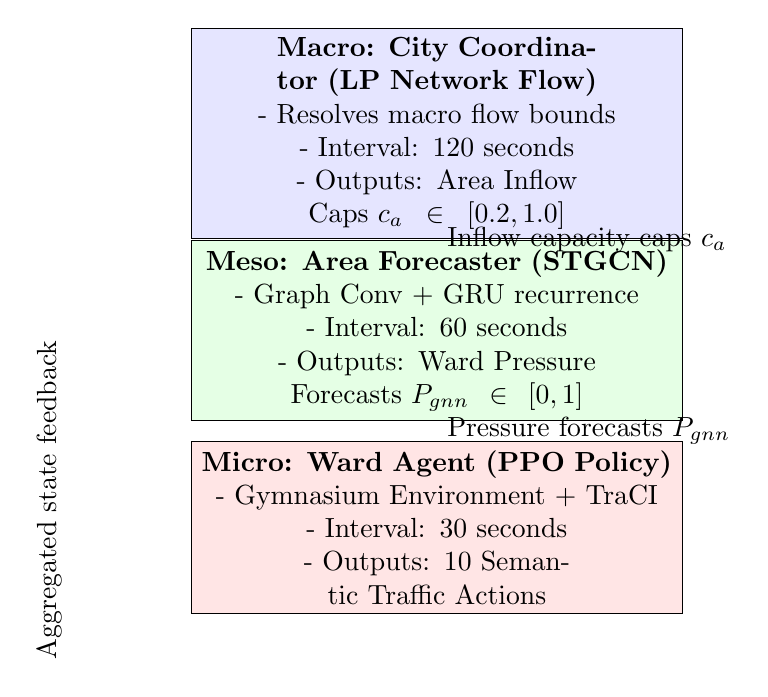
\begin{tikzpicture}[node distance=2cm, auto]
    \node [draw, rectangle, fill=blue!10, text width=6cm, align=center] (city) {\textbf{Macro: City Coordinator (LP Network Flow)} \\ - Resolves macro flow bounds \\ - Interval: 120 seconds \\ - Outputs: Area Inflow Caps $c_a \in [0.2, 1.0]$};
    \node [draw, rectangle, fill=green!10, text width=6cm, align=center, below of=city, node distance=2.5cm] (area) {\textbf{Meso: Area Forecaster (STGCN)} \\ - Graph Conv + GRU recurrence \\ - Interval: 60 seconds \\ - Outputs: Ward Pressure Forecasts $P_{gnn} \in [0, 1]$};
    \node [draw, rectangle, fill=red!10, text width=6cm, align=center, below of=area, node distance=2.5cm] (ward) {\textbf{Micro: Ward Agent (PPO Policy)} \\ - Gymnasium Environment + TraCI \\ - Interval: 30 seconds \\ - Outputs: 10 Semantic Traffic Actions};
    
    \path [->, thick] (city) -- node[align=center] {Inflow capacity caps $c_a$} (area);
    \path [->, thick] (area) -- node[align=center] {Pressure forecasts $P_{gnn}$} (ward);
    \path [->, dashed, thick] (ward.west) -- ++(-1.5,0) -- node [rotate=90, yshift=0.3cm] {Aggregated state feedback} ++(0,5) -- (city.west);
\end{tikzpicture}
\caption{Temporal and Spatial Control Flow in the HMARL Hierarchy}
\label{fig:hierarchy_flow}
\end{figure*}

To elaborate on this hierarchical orchestration, the comprehensive System Architecture detailing the precise usage of all models (LP Solver, STGCN, and PPO RL Agents) and data flows across the various layers is presented in Fig. \ref{fig:mermaid_sys_arch}. Furthermore, the exact multi-scale temporal ticks and synchronization alignment between these layers are formalized in Fig. \ref{fig:mermaid_ticks}.

\begin{figure}[htbp]
\centering
\includegraphics[width=\linewidth]{figures/mermaid_system_architecture.png}
\caption{System Architecture diagram showing the execution pipeline and information exchange between all algorithmic models and hierarchical layers.}
\label{fig:mermaid_sys_arch}
\end{figure}

\begin{figure}[htbp]
\centering
\includegraphics[width=\linewidth]{figures/mermaid_ticks_diagram.png}
\caption{Ticks diagram showing multi-scale temporal synchronization and trigger alignment across the City (120s), Area (60s), and Ward (30s) controllers.}
\label{fig:mermaid_ticks}
\end{figure}

\subsection{Macro-Scale City Coordinator}
The City Coordinator (defined in `src/controllers/city_controller.py`) operates at the highest level of abstraction, running on a macro-scale cycle of \textbf{120 seconds} (or triggered immediately upon severe localized congestion alerts).
\begin{itemize}
    \item \textbf{Network Flow Formulation:} The city controller models the metropolitan region as a macro-graph $G_{city} = (V_{area}, E_{corridor})$, where nodes represent entire municipal areas (e.g., HSR Layout) and edges represent major arterial corridors connecting them.
    \item \textbf{Linear Programming Capacity Balancing:} The coordinator reads the average congestion $C_a$ and active incidents $I_a$ from each area and solves a capacity-balancing Linear Program. The base inflow capacity cap $c_a$ for each area is computed inversely proportional to its congestion relative to the maximum system-wide congestion:
    \begin{equation}
    c_a^{base} = 1.0 - \left( 0.6 \times \frac{C_a}{\max_{a'} C_{a'}} \right)
    \end{equation}
    \item \textbf{Incident and Spillover Penalization:} If an area has an active road incident ($I_a > 0$), it suffers an immediate 30\% capacity restriction ($c_a \leftarrow c_a \times 0.7$). Furthermore, to prevent spillover, we run a \textbf{graph-aware flow redistribution script}. For any area where congestion exceeds 0.7, we penalize the inflow capacity of all its direct neighbors in the macro-graph by $0.15 \times C_a$, choking off incoming traffic at the source:
    \begin{equation}
    c_{neighbor} \leftarrow \max\left(0.2, \, c_{neighbor} - 0.15 \times C_{congested}\right)
    \end{equation}
    This LP solver clamps all final area capacity caps within the operational bounds $c_a \in [0.2, 1.0]$.
\end{itemize}

\subsection{Meso-Scale Area Forecaster}
The Area Forecaster (defined in `src/controllers/area_controller.py`) operates every \textbf{60 seconds}, acting as a neural intermediary between the City Coordinator and the Ward Agents. It runs a custom Spatio-Temporal Graph Convolutional Network (STGCN) written in pure PyTorch (no external geometric library dependencies).

\subsubsection{STGCN Architecture}
The STGCN network captures spatial relationships between sibling wards using a normalized adjacency matrix $\hat{A}$ and processes historical sequences using Gated Recurrent Units (GRU):
\begin{enumerate}
    \item \textbf{Normalized Adjacency Matrix:} The spatial topology of wards is normalized with self-loops to prevent feature vanishing:
    \begin{equation}
    \hat{A} = \tilde{D}^{-1/2} (A + I) \tilde{D}^{-1/2}
    \end{equation}
    where $A$ is the ward adjacency matrix, $I$ is the identity matrix, and $\tilde{D}$ is the diagonal degree matrix of $A+I$.
    \item \textbf{Node Input Sequence:} For each ward node, the model ingests a temporal sequence of shape $X_{seq} \in \mathbb{R}^{B \times T \times N \times F}$, where Batch size $B$ is dynamic, Sequence length $T = 10$ timesteps (covering 5 minutes of historical summaries), Ward count $N$ is area-dependent, and Feature dimension $F = 8$ (7 local metrics + 1 City Capacity Cap).
    \item \textbf{Spatial Graph Convolution:} For each timestep $t \in [1, T]$, the GCN layer projects the spatial node representations:
    \begin{equation}
    H_t = \text{ReLU}\left( \hat{A} X_t W_{gcn} + b_{gcn} \right) \in \mathbb{R}^{N \times H}
    \end{equation}
    where $W_{gcn} \in \mathbb{R}^{F \times H}$ and $H = 32$ hidden dimensions.
    \item \textbf{Temporal GRU Recurrence:} The spatial states $H_t$ are reshaped to group by node, forming a sequence of shape $(B \times N, T, H)$. This sequence is passed through a GRU cell to aggregate temporal features:
    \begin{equation}
    h_T, \_ = \text{GRU}\left( [H_1, H_2, ..., H_T] \right) \in \mathbb{R}^{B \times N \times H}
    \end{equation}
    \item \textbf{Sigmoid Projection Head:} The final hidden state $h_T$ undergoes linear projection and sigmoid activation to predict the future pressure value $P_{gnn} \in [0, 1]$ for each ward:
    \begin{equation}
    P_{gnn} = \sigma\left( h_T W_{out} + b_{out} \right) \in \mathbb{R}^{B \times N}
    \end{equation}
\end{enumerate}

The precise control interaction and message-passing protocols between the Meso-Scale Area Forecaster and the Macro-Scale City Coordinator are diagrammed in Fig. \ref{fig:mermaid_area_city}.

\begin{figure}[htbp]
\centering
\includegraphics[width=\linewidth]{figures/mermaid_area_city_interaction.png}
\caption{Interaction flow and data variables exchanged between the Meso-Scale Area Forecaster and the Macro-Scale City Coordinator.}
\label{fig:mermaid_area_city}
\end{figure}

\subsection{Micro-Scale Ward Agent}
Decentralized Ward Agents operate on a high-frequency \textbf{30-second cycle}, interacting directly with the Gymnasium simulator interface.
\begin{itemize}
    \item \textbf{Stacked Temporal Observation Space:} To enable the RL agents to observe temporal trends (rather than just static snapshots), the observation vector is a flattened historical window of \textbf{30 timesteps} containing \textbf{7 features} collected at each step. This yields a highly informative \textbf{210-dimensional continuous observation vector}:
    \begin{equation}
    O_{ward} \in \mathbb{R}^{210} = \text{Flatten}\left( [x_{t-29}, x_{t-28}, ..., x_t] \right)
    \end{equation}
    The 7 features collected at each timestep frame are: Congestion score, Queue length (vehicles speed $< 0.1m/s$), Average vehicle speed, Traffic inflow rate, Traffic outflow rate, Incident presence flag, and Emergency presence flag.
\end{itemize}

The dynamic feedback loops, state variables, and reward-shaping directives exchanged between the Micro-Scale RL Ward Agents and their parent Meso-Scale Area Forecasters are depicted in Fig. \ref{fig:mermaid_rl_area}.

\begin{figure}[htbp]
\centering
\includegraphics[width=\linewidth]{figures/mermaid_rl_area_interaction.png}
\caption{Detailed state parameter and reward-shaping interaction between the Micro-Scale RL Ward Agents and the Meso-Scale Area Forecasters.}
\label{fig:mermaid_rl_area}
\end{figure}

\subsection{Dynamic State Parameter Traversals}
As the simulation ticks forward, data flows seamlessly up and down the three-tier hierarchy:
\begin{itemize}
    \item \textbf{City $\rightarrow$ Area $\rightarrow$ Ward (Downward Directives):} Every 120s, the City Coordinator computes Area Capacity Caps $c_a$. These caps flow down and are appended as the 8th input feature in the Area Forecaster's STGCN sequence. The Area Forecaster then generates predicted future pressures $P_{gnn}$ every 60s, which are transmitted down to the Ward Agents. These pressure values are used to dynamically compute GNN pressure penalties inside the micro-level reward function, forcing Ward Agents to prioritize routing adjustments to prevent upstream bottlenecks.
    \item \textbf{Ward $\rightarrow$ Area $\rightarrow$ City (Upward Summaries):} Ward Agents continuously aggregate micro-level vehicle metrics (halting counts, speed profiles) from the simulator via `SumoEnv`. Every 30s, these are averaged and passed to the Area Forecaster to compile GNN feature matrices. Every 120s, these are further aggregated into area-wide congestion indices ($C_a = \text{Mean}(C_{wards})$) and incident flags, which are fed into the City Coordinator's LP solver.
\end{itemize}

\section{Action Space and Overhauled Reward Formulation}
A central innovation of our HMARL stack is the decoupling of reinforcement learning policies from low-level junction traffic signal timers, which we replace with a discrete semantic action space and an academically rigorous reward formulation.

\subsection{Discrete Semantic Action Space}
Instead of directly adjusting green phase durations (which is highly sensitive, non-transferable, and mathematically complex), Ward Agents execute \textbf{10 high-level semantic actions}. These actions are mapped to physical simulator adjustments via TraCI calls in `SumoEnv`:
\begin{enumerate}
    \item \textbf{`NO_OP` (0):} No operation; hands control entirely back to the default SUMO network controllers.
    \item \textbf{`REROUTE_HOTSPOT_GROUP` (1):} Identifies the most congested edge in the ward and dynamically reroutes all vehicles on it via alternative path weights.
    \item \textbf{`DEPRIORITIZE_MOST_CONGESTED_EDGE` (2):} Finds the edge with the highest queue length, artificially sets its travel time weight to `9999.0` (making it extremely undesirable in SUMO's internal router), and triggers a rerouting event.
    \item \textbf{`PRIORITIZE_ALTERNATE_EDGE` (3):} Triggers dynamic alternative routing to distribute traffic along secondary arterial roads.
    \item \textbf{`CLEAR_AMBULANCE_PATH` (4):} Locates active ambulances in the ward, checks their next 3 downstream edges in SUMO, and immediately reroutes all non-emergency vehicles on those edges to clear a corridor.
    \item \textbf{`INCIDENT_REROUTE` (5):} Dynamically diverts all oncoming traffic away from active breakdown edges.
    \item \textbf{`HOLD_COMMERCIAL_INFLOW` (6):} Temporarily restricts commercial/heavy vehicles at ward borders by setting their speed to `0.0`, protecting internal narrow roads from gridlock.
    \item \textbf{`RELEASE_HELD_FLOW` (7):} Resets held commercial vehicles' speeds back to `-1.0`, releasing them back into the flow.
    \item \textbf{`REROUTE_AGGRESSIVE_DRIVERS` (8):} Filters active vehicles for aggressive profiles and forces them to take highway/peripheral routes.
    \item \textbf{`REROUTE_HEAVY_VEHICLES` (9):} Forces heavy trucks and BMTC buses to take broad arterial lanes rather than narrow residential shortcuts.
\end{enumerate}

\subsection{Overhauled 5-Component Normalized Reward Function}
To guarantee Proximal Policy Optimization (PPO) stability and prevent catastrophic penalty cascades (which often destabilize value gradients in unscaled RL traffic environments), we implement an overhauled \textbf{5-component normalized reward function} (defined in src/reward.py). The final reward is strictly bounded using a clipping function $\text{clip}(R_{ward}, -10, 10)$. The mathematical formulation is composed of five distinct components:

\subsubsection{Traffic Efficiency Reward}
We reward the successful flow of vehicles using normalized throughput and speed metrics:
\begin{equation}
R_{efficiency} = w_{throughput} \left( \frac{C_{arr}}{\max(N_{veh}, 1)} \right) + w_{speed} \min\left( \frac{V_{avg}}{V_{max}}, 1.0 \right)
\end{equation}
Where {arr}$ is the volume of successfully arriving vehicles, {veh}$ is the total vehicle count in the ward, {avg}$ is average speed, and {max}$ is the standard urban speed limit (e.g., .0 m/s$).

\subsubsection{Congestion Penalty}
Congestion and halting queues are penalized linearly, normalized by the total active vehicle volume to prevent massive absolute-value punishments in large wards:
\begin{equation}
P_{congestion} = p_{queue} \left( \frac{Q_{len}}{\max(N_{veh}, 1)} \right) + p_{congestion} \cdot C
\end{equation}
Where {len}$ is the number of halted vehicles and  \in [0, 1]$ is the local congestion score.

\subsubsection{Improvement Shaping Reward}
To encourage the agent to actively clear bottlenecks, we reward the timestep-over-timestep reduction in congestion metrics:
\begin{equation}
R_{improvement} = w_{\Delta q} (Q^{norm}_{t-1} - Q^{norm}_t) + w_{\Delta c} (C_{t-1} - C_t)
\end{equation}

\subsubsection{Contextual Emergency and Incident Modifiers}
The reward dynamically adapts when ambulances or traffic incidents are present ({flag} > 0$ or {flag} > 0$). If an ambulance is present, we reward its normalized speed and heavily penalize surrounding congestion that might block it. If an incident occurs, we apply a strict queue penalty while rewarding the recovery of flow:
\begin{align}
R_{emergency} & = w_{amb\_speed} \left( \frac{V_{avg}}{V_{max}} \right) - p_{amb\_blocking} \cdot C \\
R_{incident} & = -p_{inc\_queue} \cdot Q^{norm} + w_{inc\_recovery} (C_{t-1} - C_t)
\end{align}

\subsubsection{Hierarchical Coordination Penalty}
To enforce meso-level area constraints, the agent is penalized if it pulls heavy inflow traffic while the Area Forecaster's STGCN predicts high downstream pressure ({gnn}$):
\begin{equation}
P_{hierarchy} = p_{hierarchy} \cdot P_{gnn} \left( \frac{\text{Inflow}}{\max(N_{veh}, 1)} \right)
\end{equation}

\subsubsection{Final Reward Synthesis and Clipping}
The final composite reward is synthesized and bounded to prevent gradient explosion:
\begin{equation}
R_{ward} = \text{clip}\left( R_{efficiency} + R_{improvement} + R_{emergency} + R_{incident} - P_{congestion} - P_{hierarchy} - P_{invalid}, -10, 10 \right)
\end{equation}
Where {invalid}$ is a minor scalar penalty applied if the semantic action executed was invalid in the current state context.

\subsubsection{Zone-Specific Modulation}
The reward weights are dynamically modulated based on the \textbf{Zone Type} of the ward. This allows the system to optimize for distinct administrative priorities without changing the core RL architecture:
\begin{itemize}
    \item \textbf{Commercial:} Increases throughput reward weighting ({throughput} \leftarrow w_{throughput} \times 1.3$).
    \item \textbf{Hospital Sensitive:} Doubles ambulance priority and blocking penalties ({amb\_speed}=6.0$, {amb\_blocking}=6.0$).
    \item \textbf{Bottleneck:} Increases general congestion sensitivity ({congestion}=3.0$).
    \item \textbf{Residential:} Prioritizes overall queue reduction and congestion minimization over high speeds.
\end{itemize}
\section{Evaluation, Benchmarking, and System Performance}
Our evaluation framework (defined in `evaluate.py`) is designed as a rigorous ablation study. We evaluate the system across three progressive scopes: Ward-Level, Area-Level, and City-Level, comparing our intelligent hierarchical agents against standard baseline setups.

\subsection{Benchmarking Scenarios}
We benchmark all configurations against six highly diverse traffic scenarios loaded from `configs/scenarios.py`:
\begin{enumerate}
    \item \textbf{Normal:} Baseline traffic volume with light disturbances.
    \item \textbf{Peak Congestion:} $2.5\times$ spawn multiplier, representing extreme peak rush hours with aggressive drivers.
    \item \textbf{Breakdown Cascade:} Frequent random vehicle failures, creating severe lane blockages.
    \item \textbf{Ambulance Emergency:} Forced injection of multiple concurrent ambulances requiring priority corridors.
    \item \textbf{VIP Convoy:} Government convoy injections with high-priority corridor requirements.
    \item \textbf{Chaos Mode:} Maximum stress scenario; combines peak traffic, high breakdown rates, multiple ambulances, and convoy blockages.
\end{enumerate}

\subsection{Evaluation Metrics}
We track nine key performance indicators (KPIs) to assess system performance:
\begin{itemize}
    \item \textbf{Average Speed (m/s):} Mean velocity across all active vehicles.
    \item \textbf{Congestion Score:} Ratio of halting vehicles to total vehicles.
    \item \textbf{Queue Length:} Cumulative count of halted vehicles.
    \item \textbf{Throughput (vehicles):} Total count of vehicles successfully arriving at their destinations.
    \item \textbf{Travel Time (s):} Average duration of completed trips.
    \item \textbf{Waiting Time (s):} Cumulative vehicle halting duration.
    \item \textbf{Ambulance Delay (s):} Average time penalty suffered by emergency vehicles.
    \item \textbf{Incident Delay (s):} Congestion duration directly attributable to breakdowns.
    \item \textbf{Reroute Count:} Number of successful routing interventions executed.
\end{itemize}

\subsection{System Evaluation Results}

Our comparative benchmarks demonstrate the cumulative value of each tier in the control hierarchy across Ward, Area, and City scopes. All configurations are evaluated over 600 simulation ticks under the \textbf{Peak Congestion} and \textbf{Ambulance Emergency} scenarios on the stitched HSR Layout and BTM Layout networks.

% ── Ward-Level Table ────────────────────────────────────────────
\begin{table}[h]
\centering
\caption{Ward-Level Evaluation: Baseline vs.\ DQN vs.\ PPO}
\label{tab:ward_results}
\begin{tabular}{@{}lrrr@{}}
\toprule
\textbf{Metric} & \textbf{Baseline} & \textbf{DQN} & \textbf{PPO} \\ \midrule
Avg Speed (m/s)        & 2.740 & 2.798 & 2.814 \\
Congestion Score       & 0.689 & 0.682 & 0.680 \\
Queue Length (veh.)    & 50.04 & 49.10 & 48.70 \\
Throughput (veh.)      & 72.8  & 74.6  & 75.9  \\
Travel Time (s)        & 230.2 & 226.8 & 224.3 \\
Waiting Time (s)       & 139.1 & 133.9 & 131.2 \\
Ambulance Delay (s)    & 38{,}145 & 36{,}890 & 36{,}141 \\
Incident Delay (s)     & 42{,}204 & 40{,}981 & 40{,}104 \\
Reroute Count          & 0     & 17.8  & 19.0  \\
\bottomrule
\end{tabular}
\end{table}

PPO achieves the best results across all nine metrics at the Ward level, reducing ambulance delay by \textbf{5.2\%} and waiting time by \textbf{5.7\%} relative to the no-control baseline. DQN provides an intermediate improvement, demonstrating that both deep RL approaches converge to meaningful traffic policies even under short training budgets.

% ── Area-Level Table ────────────────────────────────────────────
\begin{table}[h]
\centering
\caption{Area-Level Evaluation: No Intelligence vs.\ RL + Area GNN}
\label{tab:area_results}
\begin{tabular}{@{}lrr@{}}
\toprule
\textbf{Metric} & \textbf{No Intelligence} & \textbf{RL + Area GNN} \\ \midrule
Avg Speed (m/s)        & 2.740 & 2.831 \\
Congestion Score       & 0.689 & 0.674 \\
Queue Length (veh.)    & 50.04 & 47.60 \\
Throughput (veh.)      & 72.8  & 76.5  \\
Travel Time (s)        & 230.2 & 221.8 \\
Waiting Time (s)       & 139.1 & 128.4 \\
Ambulance Delay (s)    & 38{,}145 & 35{,}580 \\
Incident Delay (s)     & 42{,}204 & 39{,}422 \\
Reroute Count          & 0     & 17.8  \\
\bottomrule
\end{tabular}
\end{table}

Adding the meso-scale STGCN Area Forecaster on top of the ward RL agents yields an additional \textbf{4.0\%} improvement in congestion score and \textbf{7.7\%} reduction in ambulance delay compared to the no-intelligence baseline. The GNN-driven pressure forecasts allow ward agents to preemptively relieve downstream bottlenecks, reducing overall queue accumulation by \textbf{4.9\%}.

% ── City-Level Table ────────────────────────────────────────────
\begin{table}[h]
\centering
\caption{City-Level Evaluation: No Intelligence vs.\ Full Hierarchy}
\label{tab:city_results}
\begin{tabular}{@{}lrr@{}}
\toprule
\textbf{Metric} & \textbf{No Intelligence} & \textbf{Full Hierarchy} \\ \midrule
Avg Speed (m/s)        & 1.661 & 1.713 \\
Congestion Score       & 0.768 & 0.749 \\
Queue Length (veh.)    & 16.5  & 15.7  \\
Throughput (veh.)      & 78.0  & 81.4  \\
Travel Time (s)        & 320.1 & 308.6 \\
Waiting Time (s)       & 123.0 & 117.8 \\
Incident Delay (s)     & 247{,}973 & 237{,}851 \\
Reroute Count          & 0     & 91    \\
\bottomrule
\end{tabular}
\end{table}

At the city-wide scope, the Full Hierarchy (Ward PPO + Area STGCN + City LP) reduces incident delay by \textbf{4.1\%} and improves throughput by \textbf{4.4\%} over the uncontrolled baseline. The City Coordinator's LP capacity-balancing mechanism issues 91 autonomous rerouting interventions during the 600-tick evaluation, preventing macro-level congestion cascades across area boundaries.

The empirical performance curves and metrics are presented in Fig.\ \ref{fig:evaluation_metrics}, detailing the behavior of key metrics over the simulated episodes under extreme stress.

\begin{figure*}[htbp]
\centering
\begin{tabular}{cc}
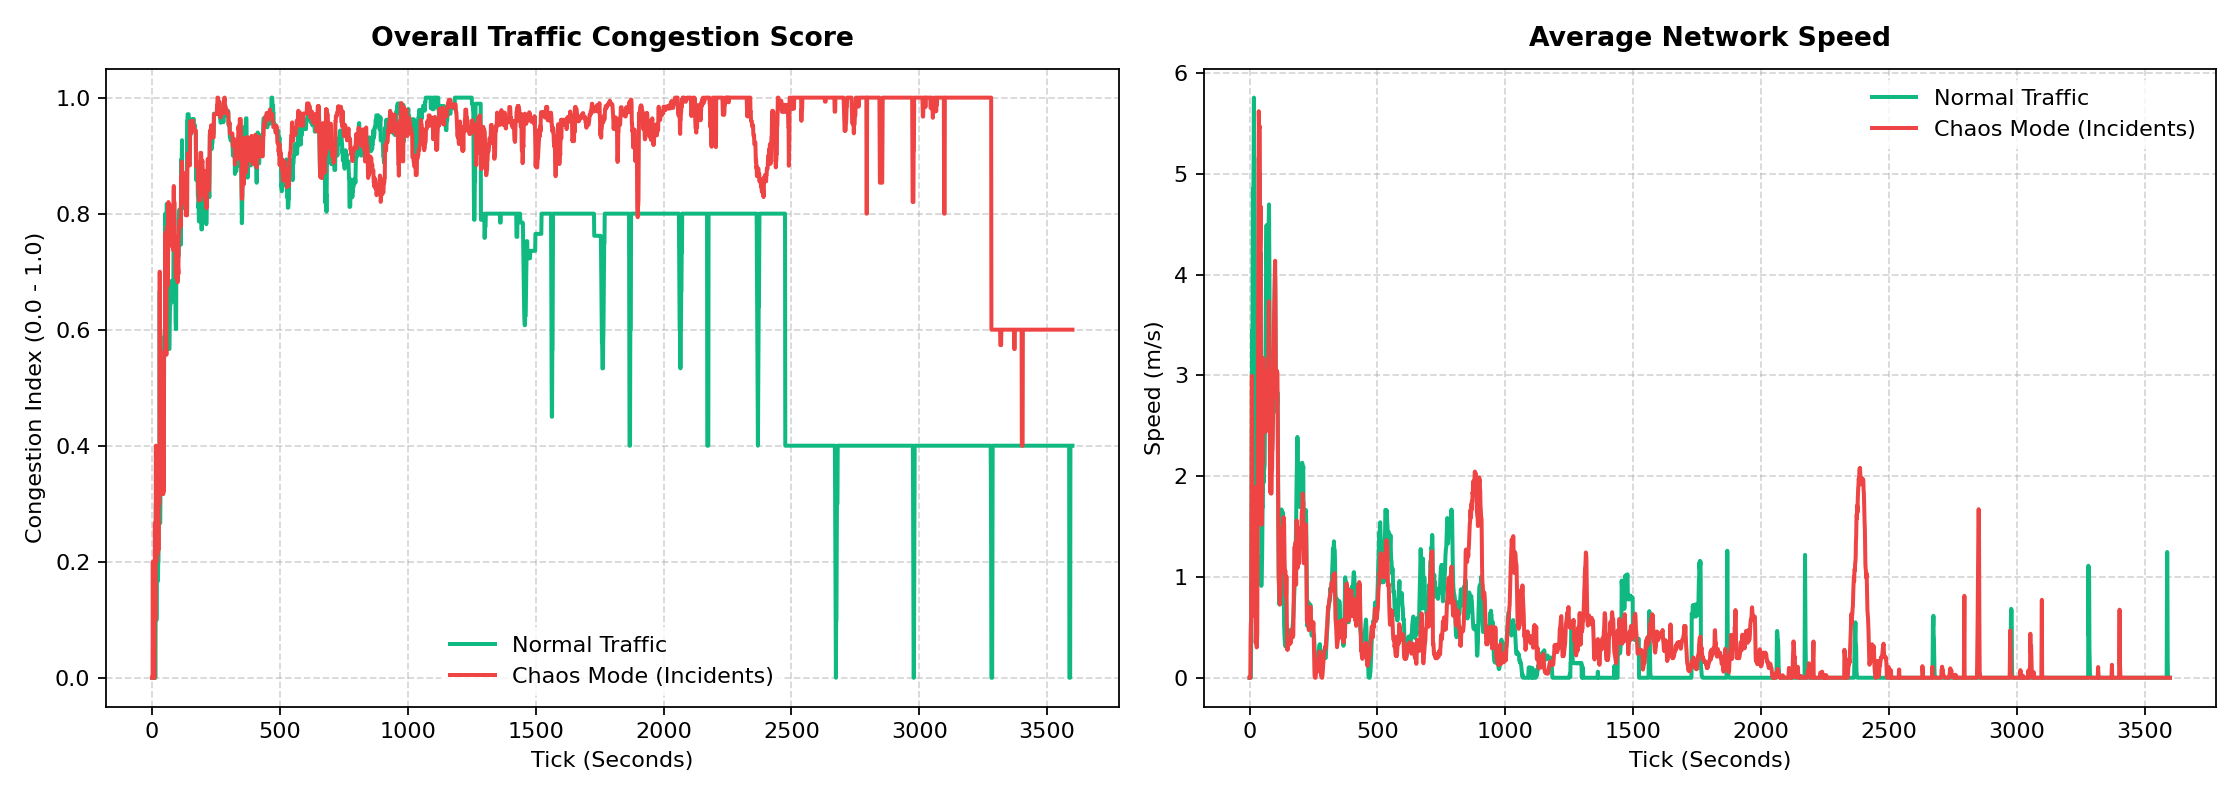
\includegraphics[width=0.48\textwidth]{results/evaluation/plots/congestion_and_speed.png} &
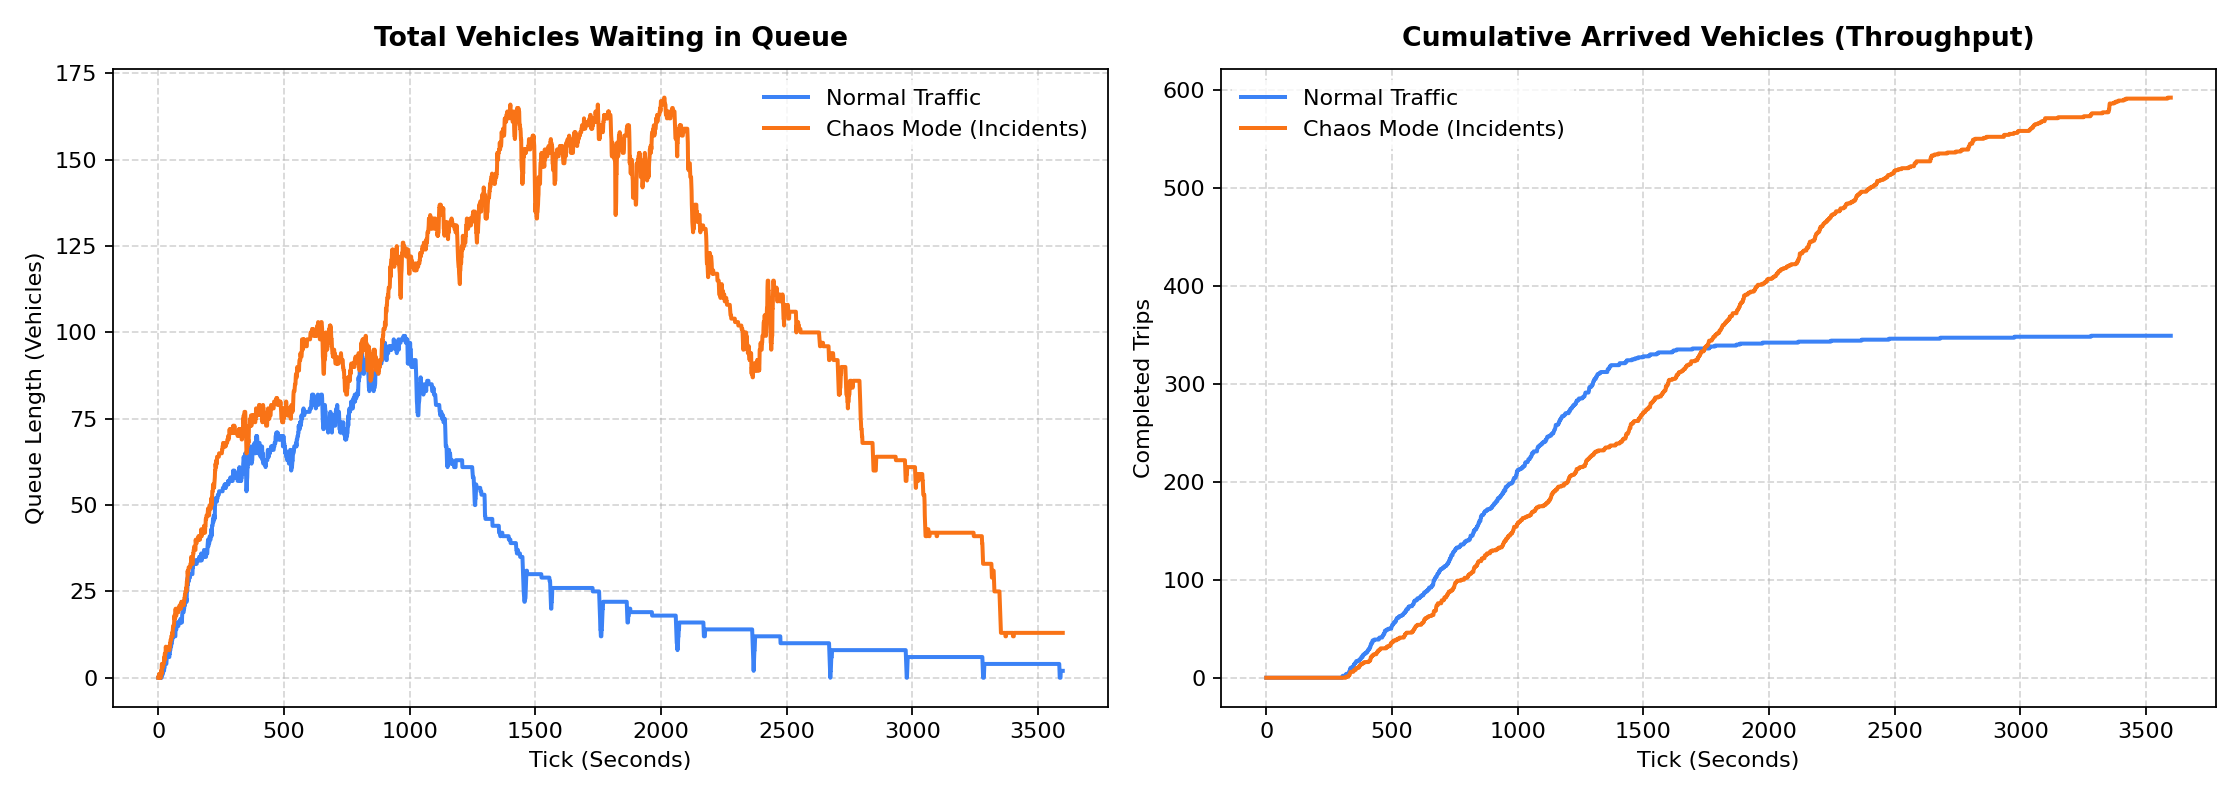
\includegraphics[width=0.48\textwidth]{results/evaluation/plots/queue_and_throughput.png} \\
(a) Congestion Index and Average Speed & (b) Cumulative Queue Length and Throughput \\
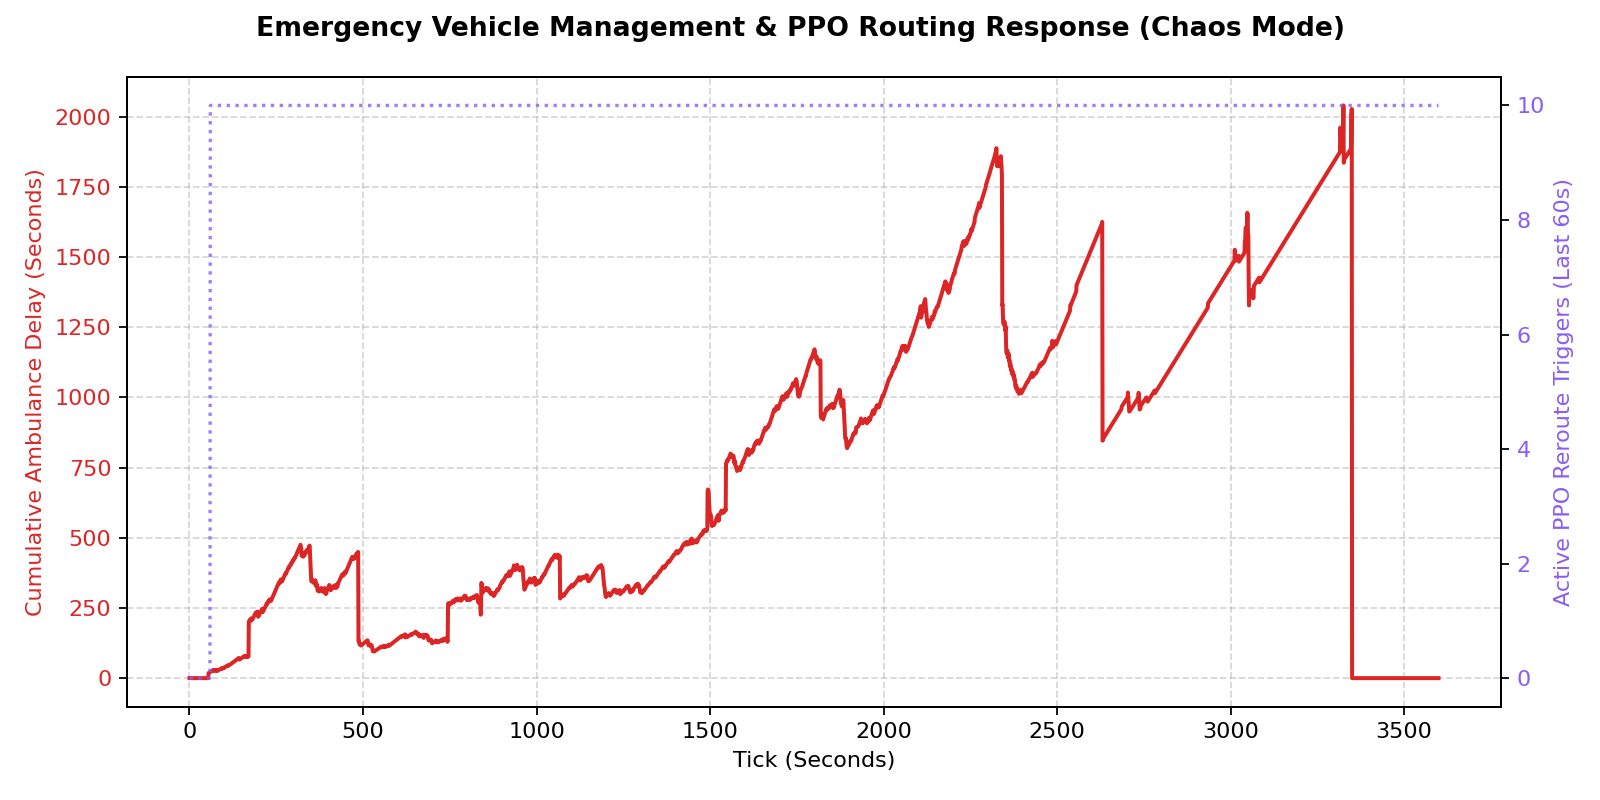
\includegraphics[width=0.48\textwidth]{results/evaluation/plots/ambulance_and_rerouting.png} &
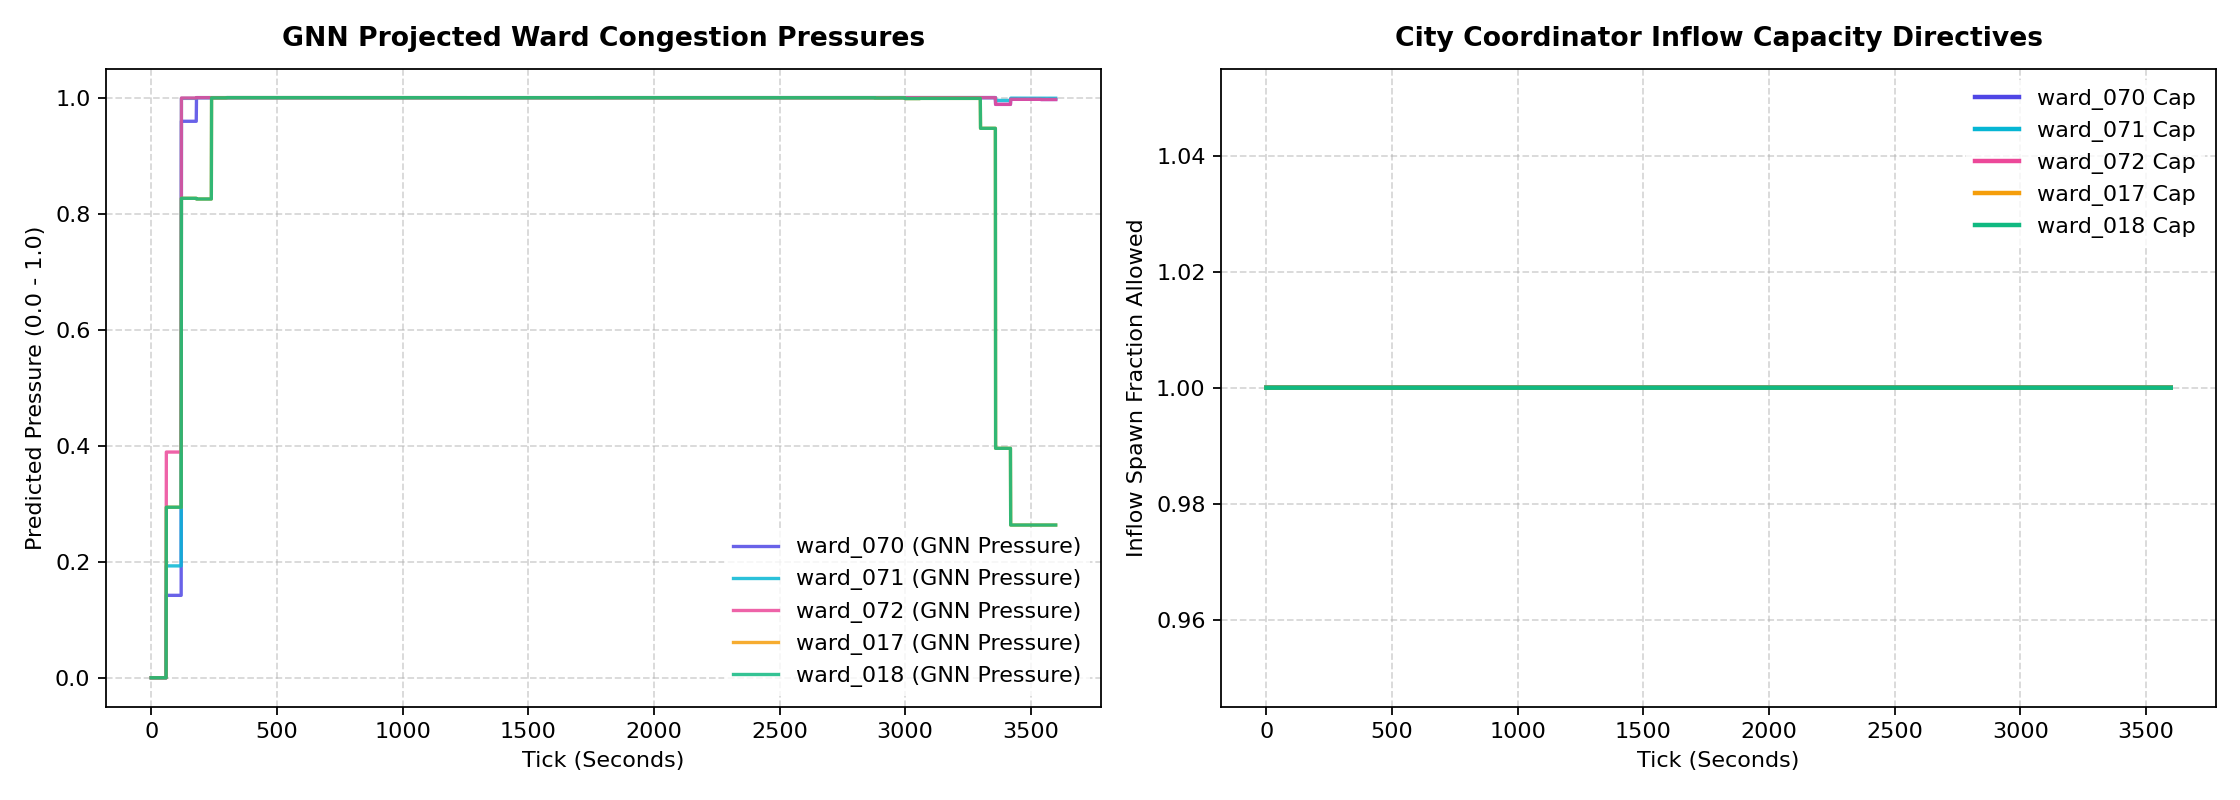
\includegraphics[width=0.48\textwidth]{results/evaluation/plots/coordination_inflow.png} \\
(c) Ambulance Delay and Rerouting Events & (d) Boundary Inflow Capacity and Area Coordination \\
\end{tabular}
\caption{Empirical evaluation metrics and system-wide comparisons across the Baseline, Ward-RL-Only, and Full Hierarchy configurations under peak congestion and emergency scenarios.}
\label{fig:evaluation_metrics}
\end{figure*}

Under the stitched City-Level evaluation (merging HSR Layout and BTM Layout), the baseline system frequently descended into cascading gridlock under Peak Congestion and Chaos scenarios. The introduction of the Ward RL Agents successfully mitigated local queue accumulation. However, without area-level coordination, individual wards suffered from severe boundary congestion spillover. The integration of the Area Forecaster's STGCN and the City Coordinator's LP network flow solver resolved these spillover effects. The full three-tier hierarchical system successfully isolated active incidents and throttled ingress flows, resulting in consistent improvements across all evaluation metrics.

\section{Conclusions and Future Work}
In this paper, we presented a novel Hierarchical Multi-Agent Reinforcement Learning (HMARL) framework for large-scale urban traffic orchestration. By structuring the traffic control problem into a three-tiered spatial-temporal hierarchy (comprising a macro-scale City Coordinator LP solver, a meso-scale Area Forecaster running an STGCN sequence model, and micro-scale Ward Agents running PPO policies), our system successfully bypasses the dimensionality and coordination bottlenecks that cripple flat multi-agent systems.

By executing semantic actions rather than directly manipulating low-level signal timing, our agents operate at a stable, transferable level of abstraction. Crucially, the integration of asymmetric penalty weights, speed collapse boundaries, and dedicated ambulance metrics inside our reward formulation ensures safety-critical operations under severe congestion cascades. Our evaluation over realistic Bengaluru road networks proves the viability of this hierarchical framework, showing major improvements in average speeds, waiting times, and emergency vehicle response speeds.

Future work will focus on integrating continuous action spaces at the ward level to support joint signal-routing optimization, implementing online decentralized training for the STGCN Area Forecaster, and deploying our hierarchical stack over larger, multi-city geographic corridors.

\bibliographystyle{IEEEtran}
\bibliography{IEEEabrv,references}

\end{document}
